% $Id: interface.tex,v 1.11 2006/09/08 23:57:16 borning Exp $

\section{Interface Design}
\label{sec:interface}

%screenshot
\begin{figure}
\centering
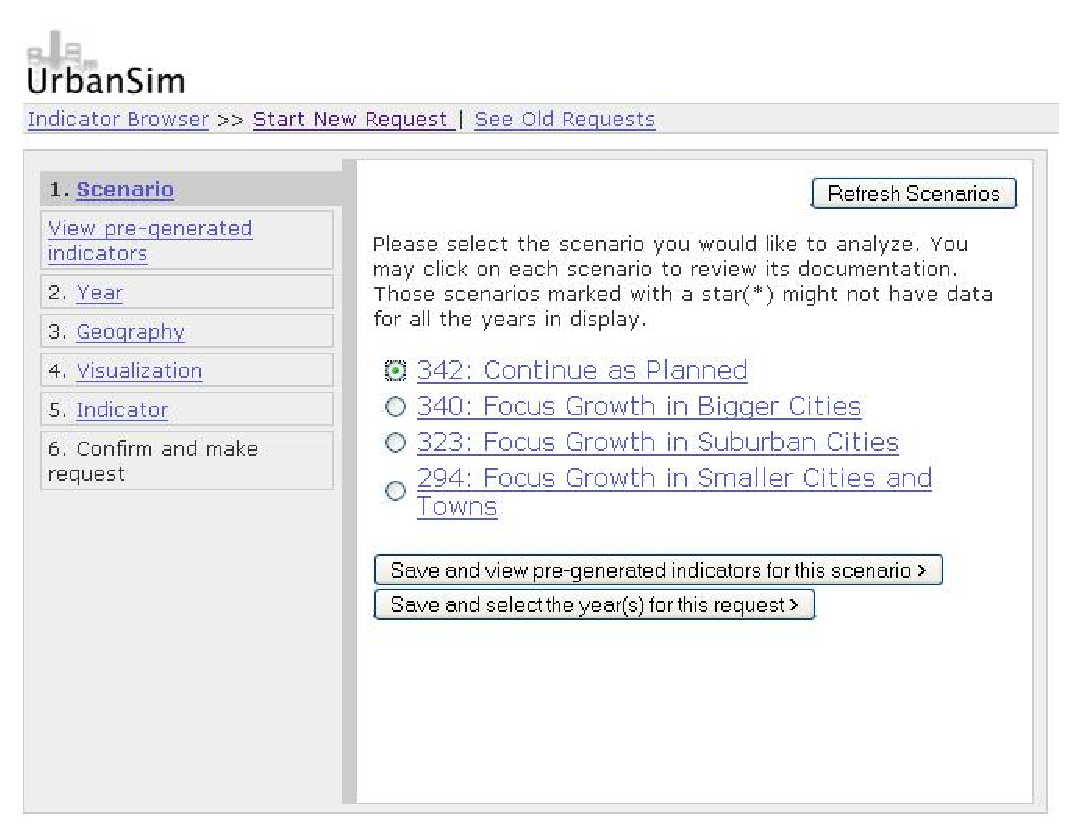
\includegraphics[width=3in]{figs/scenario_full}
\caption{\label{fig:scenario_full} Indicator Browser screenshot. The 
Session Bar on the left keeps track of users' selections and
provides easy navigation throughout the interface.}
\end{figure}

The Indicator Browser is a web-based tool for browsing through different
UrbanSim runs, and indicator values that have already been computed for those
runs and their visualizations.  It also allows new indicator values and
visualizations to be requested, using a web-based form. It is
intended to make indicators easier to generate by the interface's target users. 
It is also intended as a 
step towards including more of the indirect stakeholders into
the direct stakeholder group.  Its design and implementation is strongly
informed by the Value Sensitive Design work, in particular, the empirical
results on the usefulness of providing tools that contain ready-to-hand information, and on
transparency.

In addition, the design and testing of the Indicator Browser made extensive
use of user-centered design techniques, including iterative design, paper
prototyping, and frequent design discussions and user feedback.  
The intended users
are urban modelers and planners, as well as software developers.  Each
iteration was designed and evaluated using interactive or paper prototypes
keeping in mind the values that UrbanSim is meant to explicitly support.  A
brief description of all these methodologies, as well as their specific
application for the Indicator Browser, follow below.

\subsection{Iterative User Interface Design}

Iterative user interface design is by now standard practice in the Human Computer
Interaction (HCI)
community (see e.g.\ \cite{nielsen-ieee-computer-1993}).  It is based on
the realization that even the best designers will not design the ideal
interface on the first attempt; instead, iterative testing, feedback, and
refinement is essential in order to determine where and how to allocate
design efforts.  There is a continuing cycle of design, testing, and
feedback to the design.

%results page and session bar
\begin{figure}
\centering
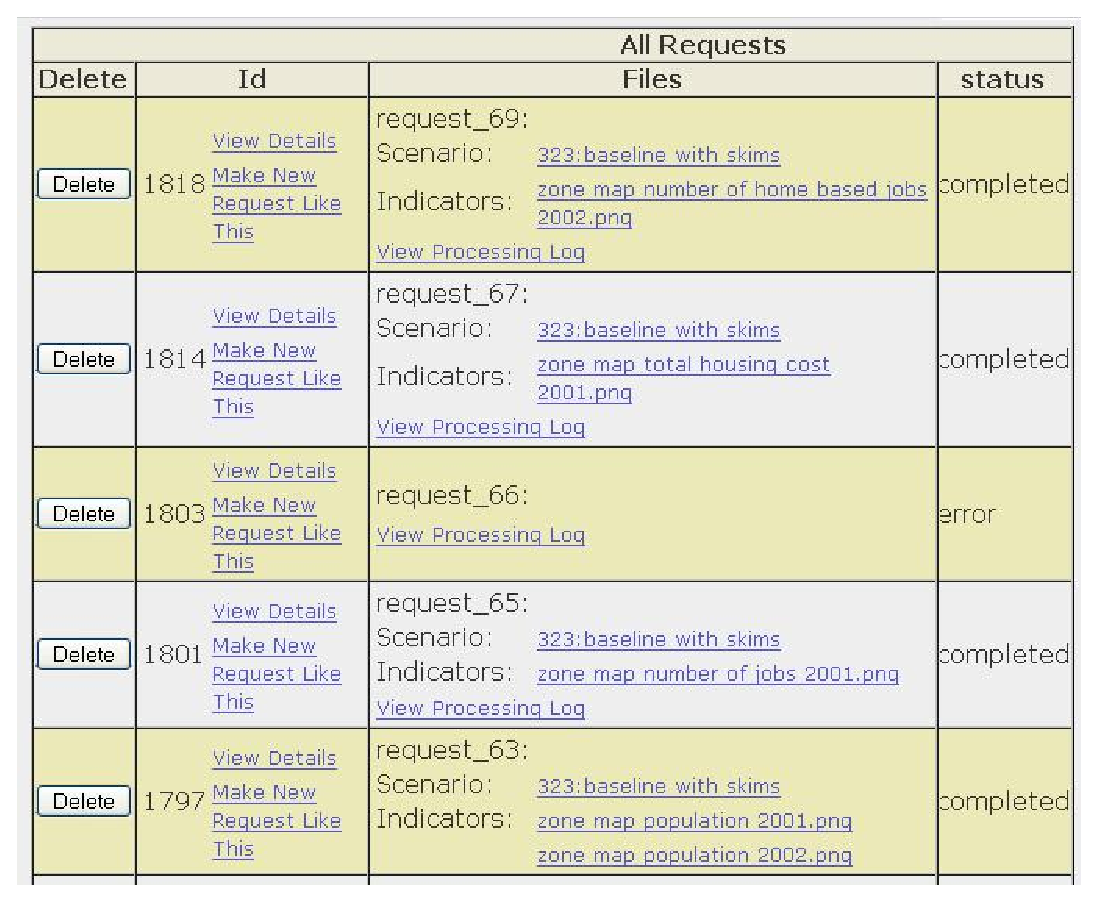
\includegraphics[width =3in]{figs/results}

\caption{\label{fig:results} Results Page, which contains
information about current as well as previous requests, and provides
commands to view details, delete requests, and make requests like
previous ones.}
\end{figure}

\subsection{Paper prototyping}

%scenario indicator and years page
\begin{figure*}
\centering
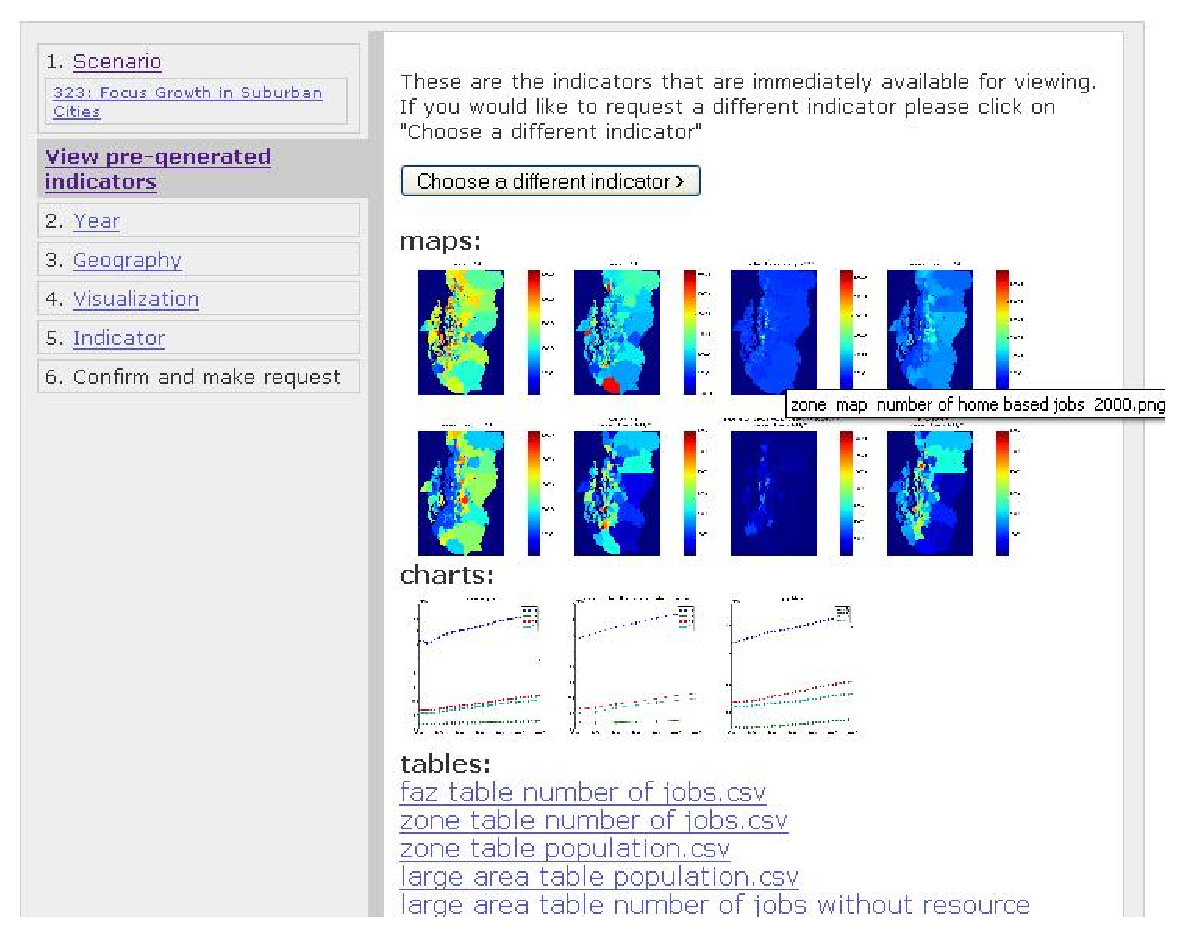
\includegraphics[width=7in]{figs/pregenerated}

\caption{\label{fig:pregenerated} Pre-generated
Indicators page, which displays all the indicators that are immediately
available for viewing.}
\end{figure*}

Paper prototyping originated in the Participatory Design work in
Scandinavia in the 1970s and 80s \cite{greenbaum-pd-1991}, but has since
become widely used as part of iterative user interface design techniques
\cite{rettig-cacm-1994}.  It is used to evaluate interfaces in the early
stages of the design process, with the goal of fixing as many usability
problems as possible before implementing the system. Although there are
certain interface affordances that paper prototypes simply cannot capture
(such as the experience of clicking a button), addressing design decisions
such as selecting feature sets and basic user-interface interactions using
paper prototypes lowers the design and implementation costs while having
tremendous impacts on the usability of the interface
\cite{nielsen-alertbox-paper-prototyping}.

The Indicator Browser design process combined usability testing,
iterative user-interface design via paper prototyping, and the Value
Sensitive Design methodology.  The principal goal in the Indicator Browser
design work has been for it to be usable by the target users
while continuing to support UrbanSim's core values.

\subsection{The Design Process} 

The Indicator Browser was designed through iterative user-interface design.
There was an informal initial discussion with modelers and planners at the
PSRC, which resulted in an initial sketch of the interface.  This interface
would be a single web page that would let users select the scenario that
they wished to visualize, along with specifications about the
visualization, such as its type, years, geography and of course, the
indicator(s) selection. After some technical investigations, the designers
found the implementation of this interface challenging due to the
dependencies between these selections, which are discussed 
in the next section. Therefore, the
designers moved to a sequential interface, in which the user's choices on
one web page would affect the content and available options for subsequent
pages.  The first author then performed a small informal interface
evaluation and fixed some usability issues to get the interface ready for
user interface evaluations.

Finally, two rounds of interface evaluations using rapid paper prototyping
were performed with eight urban modelers and planners at UrbanSim and
PSRC in May and June of 2005, respectively. A team of researchers
designed paper prototypes by printing the already existing Indicator
Browser web pages, sketching new pages using pencil and paper, and using
common stationary such as double-sided tape or stickers to create paper
widgets, for instance, drop-down menus or radio button selections.  The
interface design was refined by using the paper prototype to attempt to
complete a set of representative tasks. The tasks were developed using
personas that represented our target users, using the knowledge that some
of the researchers in the design team had about urban planning and our
target users.

The design team proceeded to evaluate the interface with volunteer
evaluators at PSRC and UrbanSim. As is usual with paper prototypes, one
person in the design team acted as a computer by reacting to user input
while the rest of the team recorded the user's experience. We asked our
users to think aloud, to say whatever was on their mind when they were
using the interface, in order to determine the interface's usability. We
were especially interested in determining which parts of the interface
worked well, so that we wouldn't alter them during the next round of
design, and which parts of the interface were confusing, in order to come
up with better design alternatives. In addition, we got suggestions
regarding the representative tasks, which we refined as well through the
multiple evaluations.  After the user completed the representative tasks we
asked them if they had any general suggestions and we explored possible
design alternatives together.
  
%\input{firsteval}

%\input{secondeval}

% LocalWords:  borning UrbanSim VSD UrbanSim's design's Habermas affordances UI
% LocalWords:  PSRC personas HCI yaels screenshot Pre
